\documentclass[UTF8]{ctexart}
\usepackage{anyfontsize}
\usepackage{geometry}
    \geometry{left=4cm,right=4cm,top=2cm,bottom=2cm}
\usepackage{amsmath, amssymb, amsthm}
\usepackage{caption} 	 % 标题
\usepackage{xcolor} 	 % 颜色
\usepackage{graphicx} 	 % 引用图片
\usepackage{float}
\usepackage{indentfirst} 	 % 首行缩进 
    \setlength{\parindent}{0em}
\usepackage{setspace} 	 % 行间距 \begin{spacing}{arg}
\usepackage{esvect} 	 % 向量箭头 \vv{}
\usepackage{esint} 	 % 积分符号
\usepackage[italic=true]{derivative}

\pagestyle{empty}

\begin{document}
\section{常用积分表}
注: 常数 $ C $ 省略.

\subsection{基本}
$ \displaystyle d x = \dfrac{d(ax + b)}{a} \hspace{5em} \int f(ax + b) \,dx = \dfrac{1}{a} \int f(ax + b) \,d(ax + b) $

\subsection{有理函数 / 部分分式}
若 $ \Delta > 0 $, 方程两根分别记作 $ x_1 = \dfrac{-b + \sqrt{\Delta}}{2a} $, $ x_2 = \dfrac{-b - \sqrt{\Delta}}{2a} $.
\vskip 0.5em

$ \displaystyle
    \int \dfrac{1}{ax^2 + bx + c} \,dx =  \begin{cases}
        \dfrac{2}{\sqrt{-\Delta}} \arctan \dfrac{2ax + b}{\sqrt{-\Delta}} \qquad, \Delta < 0 \\[1em]
        \dfrac{1}{\sqrt{\Delta}} \ln \left| \dfrac{x - x_1}{x - x_2} \right| = \dfrac{1}{a(x_1 - x_2)} \ln \left| \dfrac{x - x_1}{x - x_2} \right|  \qquad, \Delta > 0
    \end{cases}
$
\vskip 1em


$ \displaystyle \int \frac{x}{ax^2 + bx + c}\,dx = \frac{1}{2a} \ln \left| ax^2 + bx + c \right| - \frac{b}{2a} \int \frac{dx}{ax^2 + bx + c}  $
\vskip 1em

$ \displaystyle \int \dfrac{dx}{(ax^2 + bx + c)^n} \ (\Delta < 0) $ 总是可以通过配方和换元化为 $ J_n $.
\vskip 1em

$ \displaystyle J_n = \int \dfrac{dx}{(x^2 + a^2)^n} $, 作换元 $ \dfrac{1}{(x^2 + a^2)^n} = t $, 运用分部积分法 $ \int t \,dx = tx - \int x \,dt $, 可以找到 $ J_{n + 1} $ 到 $ J_n $ 的递推式, 而 $ \displaystyle J_1 = \dfrac{1}{a} \arctan \dfrac{x}{a} $.

\subsection{一些基本积分}
$ \displaystyle I_1 =  \int \dfrac{dx}{a^2 + x^2} = \dfrac{1}{a}\arctan \dfrac{x}{a} $
\hskip 4em
$ \displaystyle I_2 = \int \dfrac{dx}{\sqrt{a^2 - x^2}} = \arcsin \dfrac{x}{a} $
\vskip 1em

$ \displaystyle I_3 = \int \dfrac{dx}{\sqrt{x^2 \pm a^2}} = \ln \left|x + \sqrt{x^2 \pm a^2}\right|  $
\vskip 1em

$ \displaystyle I_4 = \int \dfrac{dx}{\sqrt{a x^2 + b x + c}} $
\hskip 4em
$ \displaystyle I_5 = \int \sqrt{a x^2 + b x + c} \,dx $
\vskip 1em

对于 $ I_4 $, 当 $ a > 0 $ 时, 将二次三项式配方成为 $ a \big[ (x + \alpha)^2 \pm \beta^2 \big] $ 的形式, 于是转化为 $ I_3 $; 当 $ a < 0 $, 配方得到 $ -a \big[ \beta^2 - (x + \alpha)^2 \big] $, 于是转化为 $ I_2 $.
\vskip 1em

对 $ \displaystyle I_5 $ 使用分部积分得到关于 $ I_5 $ 和 $ I_4 $ 的方程, 于是可以解出 $ I_5 $ 转化为 $ I_4 $.


\subsection{三角函数积分/导数}

$ (\tan x)' = \sec^2 x \qquad (\cot x)' = -\csc^2 $
\vskip 1em

$ (\sec x)' = \sec x \tan x \qquad (\csc x)' = - \csc x \cot x $
\vskip 1em

$ \displaystyle \int \tan x \,dx = - \ln |\cos x| $, $\quad$ ($ \tan $ 分母为 $ \cos $)
\vskip 1em

$ \displaystyle \int \cot x \,dx = \ln |\sin x| $, $\quad$ ($ \cot $ 分母为 $ \sin $)
\vskip 1em

$ \displaystyle \int \sec x \,dx = \ln |\sec x + \tan x| = \ln \left| \tan \left( \dfrac{x}{2} + \dfrac{\pi}{4} \right) \right| $
\vskip 1em

$ \displaystyle \int \csc x \,dx = \ln |\csc x - \cot x| = \ln \left| \tan \dfrac{x}{2} \right| $

\subsection{表格法}
$ \displaystyle \int f(x) e^{ax} \,dx = e^{ax} \left[ \dfrac{f(x)}{a} - \dfrac{f'(x)}{a^2} + \dfrac{f''(x)}{a^3} - \dfrac{f'''(x)}{a^4} + \dfrac{f^{(4)}(x)}{a^5} - \cdots \right] $
\vskip 1em

% $ \displaystyle \int f(x) \sin ax \,dx $ 或 $ \displaystyle \int f(x) \cos ax \,dx $ 也可采用表格法, 通常 $ f(x) = x^n $

$ \displaystyle \int \ln^m x \cdot x^n \,dx $ 作换元 $ \ln x = t $ 得 $ \displaystyle \int t^m \cdot e^{(n+1)t} \,dt $

\subsection{竖线记号}
\begin{itemize}
    \item 线性: $ \big[ C \cdot f(x) \big]_a^b = C \cdot \big[ f(x) \big]_a^b \hspace{3em} \big[f(x) \pm g(x) \big]_a^b = \big[f(x)\big]_a^b \pm \big[g(x) \big]_a^b $
    \item 反对称: $ -\big[f(x)\big]_a^b = \big[f(x)\big]_b^a $
\end{itemize}


\section{积分技巧}
\subsection{定积分}
\begin{enumerate}
    \item $ f(x) $ 为奇函数 (拆分成 $ \int_{-a}^{0} + \int_{0}^{a} $, 对第二个作替换 $ x = a - t $): \[ \int_{-a}^{a} f(x) \,dx = 0 \]
    \item $ f(x) $ 为偶函数 (同上): \[ \int_{-a}^{a} f(x) \,dx = 2 \int_{0}^{a} f(x) \,dx \]
    \item 三角函数 (分别作替换 $ x = \pi/2 - t $ 以及 $ x = \pi - t $): \[ \int_{0}^{\pi/2} f(\sin x) \,dx = \int_{0}^{\pi / 2} f(\cos x) \,dx \]\[ \int_{0}^{\pi} x f(\sin x) \,dx = \dfrac{\pi}{2} \int_{0}^{\pi} f(\sin x) \,dx \]
    作相同的替换, 可以得到上面两式的推广: \[ \int_{0}^{\pi/2} f(\sin x, \cos x) \,dx = \int_{0}^{\pi/2} f(\cos x, \sin x) \,dx \] \[ \int_{0}^{\pi} x f(\sin x, \cos x) \,dx = \dfrac{\pi}{2} \int_{0}^{\pi} f(\sin x, -\cos x) \,dx \]
     \item 周期函数: $ f(x) $ 的周期为 $ T $, 则任何长度为 $ T $ 的区间上的积分都相等: \[ \int_{a}^{a+T} f(x) \,dx = \int_{0}^{T} f(x) \,dx \]
    \item Wallis' Integral:
          \[ \int_{0}^{\pi/2} \sin^n x \,dx = \int_{0}^{\pi/2} \cos^n x \,dx =
              \begin{cases}
                  \dfrac{(n - 1)!!}{n!!}\cdot \dfrac{\pi}{2} & , n \text{ 为偶数} \\[1em]
                  \dfrac{(n - 1)!!}{n!!}                     & , n \text{ 为奇数}
              \end{cases}
          \]
    \item Wallis' Integral 推广:
          \[ \int_{0}^{\pi/2} \sin^n x \cos^m x \,dx =
              \begin{cases}
                  \dfrac{(n - 1)!! (m - 1)!!}{(m + n)!!} \cdot \dfrac{\pi}{2} & , \text{$ n $ 和 $ m $ 为偶数} \\[1em]
                  \dfrac{(n - 1)!! (m - 1)!!}{(m + n)!!}                      & , \text{ 其余情况}
              \end{cases}
          \]
    \item 与求和 $ (\sum) $ 类似的积分区间平移: \[ \int_{I} f(x) \,dx = \int_{I \pm k} f(x \mp k) \,dx \]
    \item 幂函数乘上对数 (分部积分):
    \[ \int_0^1 x^k \ln^m x \,dx = \dfrac{(-1)^m \cdot m!}{(k+1)^{m+1}} \]
\end{enumerate}

\vskip 2em
\subsubsection{对称性}
定义域关于原点对称, $ f(x) $ 和 $ f(-x) $ 积分相同:
\begin{align} \label{eq:1}
    \int_{-a}^{a} f(x) \,dx = \int_{-a}^{a} f(-x) \,dx 
\end{align}

所以有:
\[ 
    \int_{-a}^{a} f(x) \,dx = \int_{-a}^{a} \dfrac{f(x) + f(-x)}{2} \,dx = \int_{0}^{a} \big[ f(x) + f(-x) \big] \,dx   
\]
注意 $ f(x) + f(-x) $ 为偶函数.
\vskip 2em

可将 \eqref{eq:1} 推广至任意区间:
\[ \int_{a}^{b} f(x) \,dx = \int_{a}^{b} (a + b - x) \,dx \]

\begin{figure}[H]
    \centering
    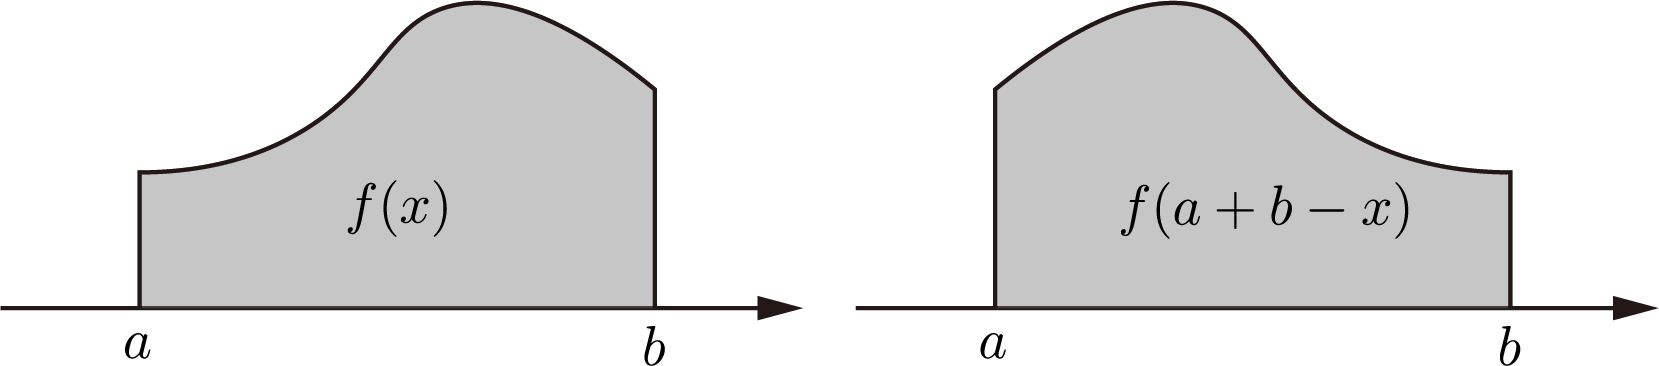
\includegraphics[width = 0.8\linewidth]{symmetry1}
\end{figure}


\paragraph{例}
\[ \int_{0}^{r} x^m (r - x)^n \,dx = \int_{0}^{r} x^n (r - x)^m \,dx \]


\vskip 3em
\subsection{二重积分}
\begin{enumerate}
    \item 常数: \[ \displaystyle \int_D C \,dx\,dy = m(D) \]
    \item 部分可加(要求参与并集运算的两个区间互斥): \[ \int_Y \int_{X_1} f \,dx\,dy + \int_Y \int_{X_2} f \,dx\,dy = \int_Y \int_{X_1 \cup X_2} f \,dx\,dy \]\[ \int_{Y_1} \int_{X} f\,dx\,dy + \int_{Y_2}\int_{X} f\,dx\,dy = \int_{Y_1 \cup Y_2} \int_X f \,dx\,dy \]
\end{enumerate}

\begin{figure}[H]
    \centering
    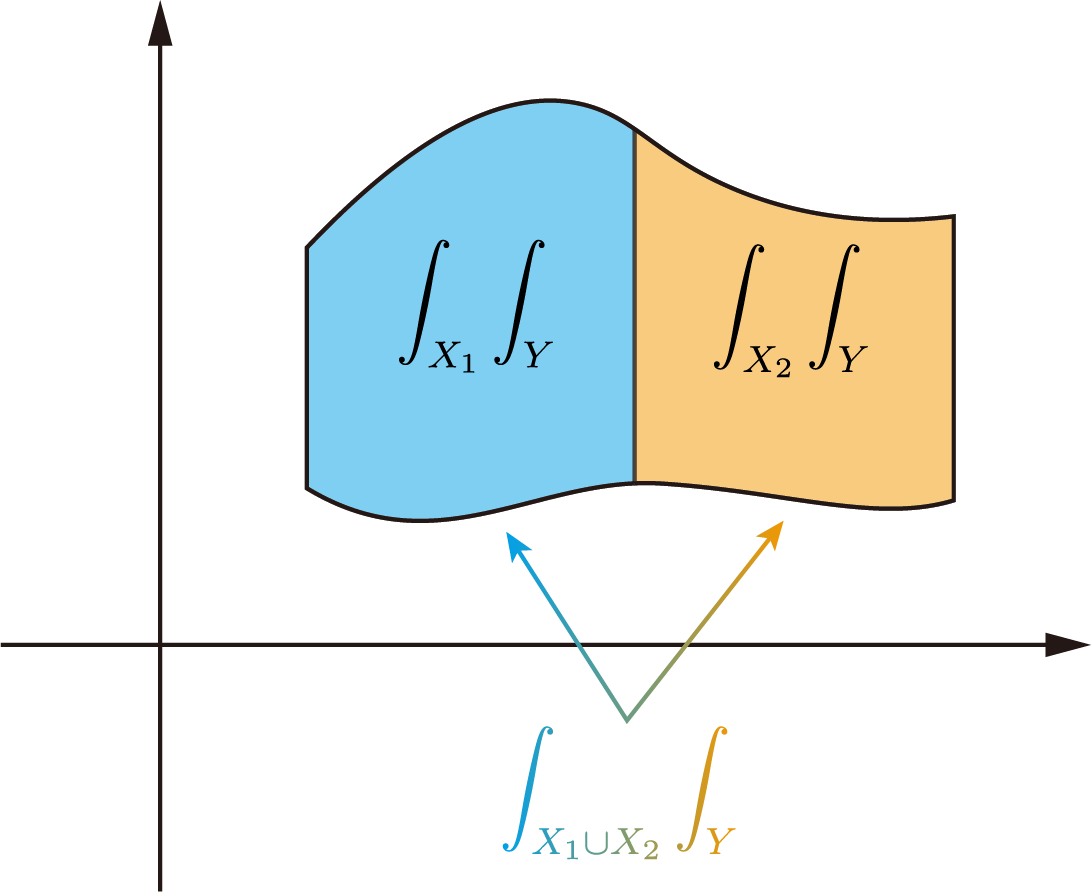
\includegraphics[width = 0.5\linewidth]{region_additive}
    \caption*{区域部分可加性图解}
\end{figure}


\subsubsection{对称性}
类似于一元函数定积分, 当区域具有对称性时, 区域上二重积分也有一定性质:

当 $ f $ 是关于 $ x $ 或 $ y $ 的奇/偶函数, 可参考一元函数定积分相关性质.

\begin{enumerate}
    \item 定义域关于 $ x $ 轴对称, 将函数沿 $ x $ 轴面对称, 积分不变 \[ \iint_D {\color{red} f(x, y)} \,dx\,dy = \iint_D {\color{blue} f(x, -y)} \,dx\,dy \]
    \item 定义域关于 $ y $ 轴对称, 将函数沿 $ y $ 轴面对称, 积分不变 \[ \iint_D {\color{red} f(x, y)} \,dx\,dy = \iint_D {\color{blue} f(-x, y)} \,dx\,dy \]
    \item 定义域关于原点对称, 将函数沿原点轴对称, 积分不变 \[ \iint_D {\color{red} f(x, y)} \,dx\,dy = \iint_D {\color{blue} f(-x, -y)} \,dx\,dy \]
    \item 定义域关于 $ y = x $ 对称, 将函数沿 $ y = x $ 面对称(交换 $x$,$y$), 积分不变 \[ \iint_D {\color{red} f(x, y)} \,dx\,dy = \iint_D {\color{blue} f(y, x)} \,dx\,dy \]
\end{enumerate}

\begin{figure}[H]
    \centering
    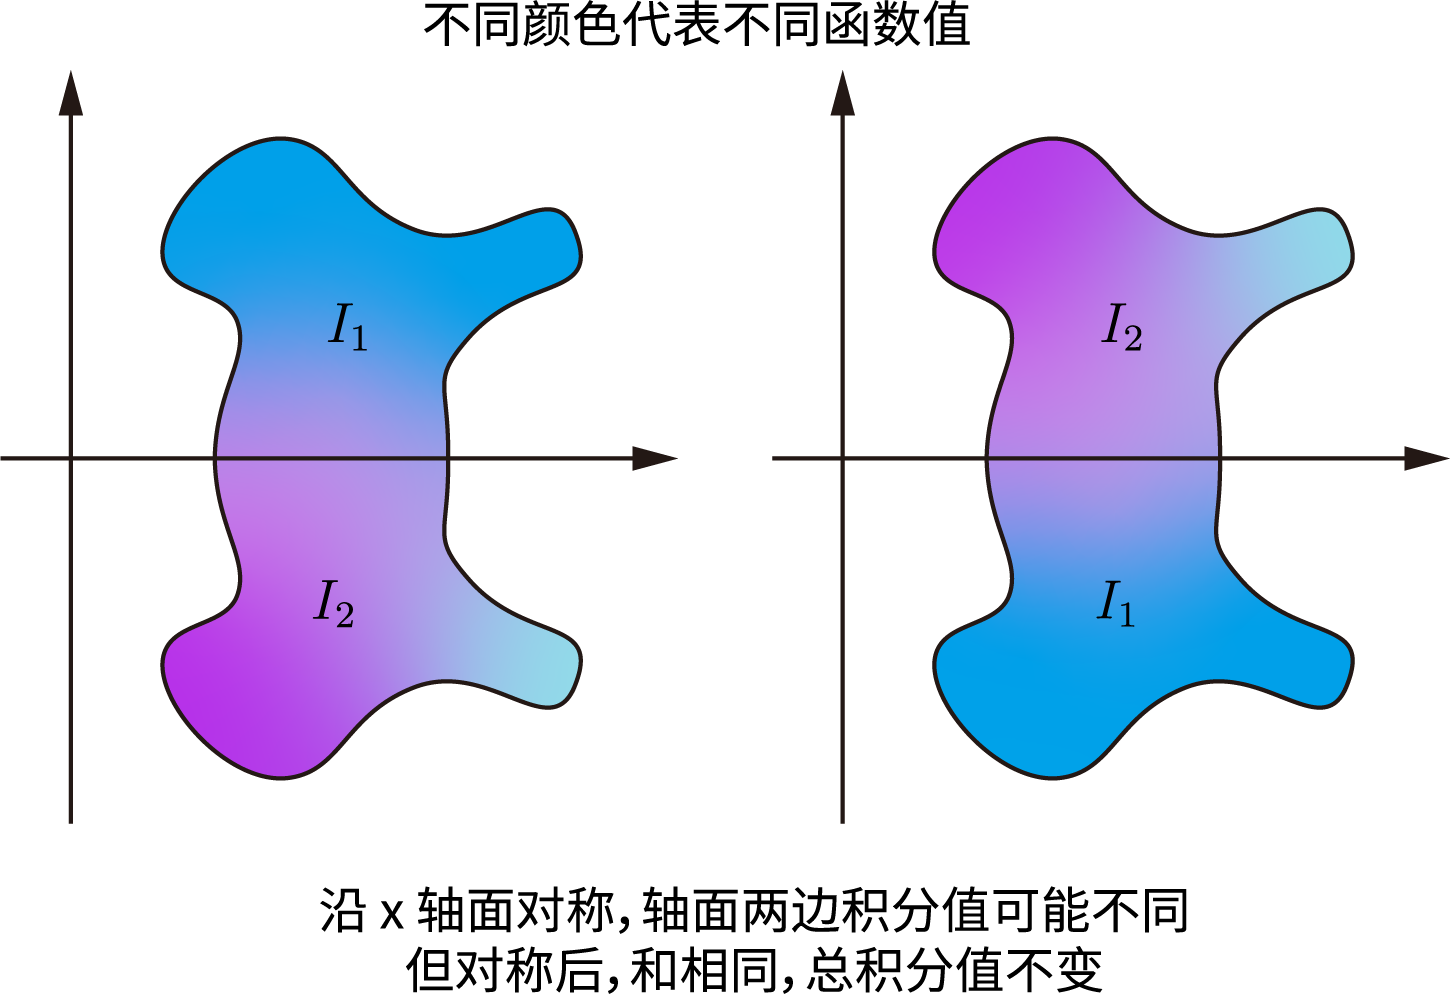
\includegraphics[width = 0.65\linewidth]{symmetry2}
\end{figure}



\end{document}